\section{Acceptance X Efficiency}
\label{sec:AccXEff}

Computed as a combined value; Based on the signal MC

The numerator:

For the total cross section: selected signal MC yields with PU weight applied
For differential cross section: selected signal MC yields with PU weight applied in $P_T^{\gamma-GEN}$ bins 15-20-25... Transition to the$P_T^{\gamma-RECO}$ bins is performed by unfolding

The denominator:

For each event in unskimmed signal MC file, photon and lepton which refer to W$\gamma$ and determine $\Delta R^{gen}$ and $P_T^{\gamma-gen}$ 
For the total cross section: calculate number of events within phase space cut\\
For the differential cross section: calculate number of events within phase space cut in 15-20-25-30-35-45-55-65-75-85-95-120-500 GeV $phoEt_{gen}$ bins

accXeff are computed and applied together as a bin-by-bin correction
accXeff on total yield is:
Electron channel: accXeff Tot=(21833$\pm$36)/(177606$\pm$629)=0.1229$\pm$0.0004
Muon channel: accXeff Tot=(51771$\pm$39)/(179082$\pm$631)=0.2891$\pm$0.0006
\begin{figure}[htb]
  \begin{center}
  \includegraphics[width=0.5\textwidth]{../figs/figs_v11/MUON_WGamma/Constants/C_accXeff_MUON_WGamma.pdf}\includegraphics[width=0.5\textwidth]{../figs/figs_v11/ELECTRON_WGamma/Constants/C_accXeff_ELECTRON_WGamma.pdf}\\
  \label{fig:covMatricesaccXeff_Wg}
  \end{center}
\end{figure}

%\begin{figure}[htb]
%  \begin{center}
%     \includegraphics[width=0.48\textwidth]{figs_v8/MUON_WGamma/Constants/C_accXeff_MUON_WGamma.pdf} \includegraphics[width=0.48\textwidth]{figs_v8/ELECTRON_WGamma/Constants/C_accXeff_ELECTRON_WGamma.pdf}
%  \caption{Acceptance X Efficiency. Left: MUON channel, right: electron channel.}
%  \label{fig:accXeff_Wg}
% \end{center}
%\end{figure}

The Phase Space Definition:
%  Applied at generator-level to compute acceptance and MC-based cross section;\\
  (tried to follow to the phase space definition of the approved Z$\gamma$ analysis [AN-2013-280] as close as possible)
  \begin{itemize}
  \item $p_T^{\gamma}$ $>$ 15 GeV
  \item $\Delta{R}(\gamma,lep) > 0.7$
  \item $|\eta^{\gamma}|<2.5$, $|\eta^{lep}|<2.5$
  \item $p_T^{lep}>$ 20 GeV
  \item $Iso^{\gamma}<$ 5 GeV (sum of all $P_T$ within $\Delta{R}<$0.3 based on MC-generated particles)
%  \item for Z$\gamma$ Check: M(lep,lep)$>$50 GeV
  \item for differential cross section, $P_T^{\gamma}$ binning: 15-20-25-30-35-45-55-65-75-85-95-120-500 GeV
  \end{itemize}

To determine whether the event within the phase space or not, the following algorithm was used:
\begin{itemize}
   \item find a muon/electron which has a W boson as a mother particle
   \item add 4-momenta of the dressing photons to the 4-momentum of the muon/electron; dressing photons as defined as photons that have $P_T>0.5$ GeV and have $\Delta R(lepton,photon)<0.1$
   \item find a final state photon which corresponds to FSR, ISR or TGC; exclude dressing photons from the consideration
   \item using 4-momentum of the photon and the adjusted 4-momentum of the lepton, determine whether the event is within the phase space or not
\end{itemize}

